\documentclass[a4paper,11pt]{article}
\usepackage[utf8]{inputenc}
\usepackage[francais]{babel}
\usepackage{graphicx}
\usepackage{fancyhdr}

% Title Page
\title{SPAM ASSASSIN}
\date{Décembre 2014}
\author{Mathieu KERN -}
\pagestyle{fancy}


\begin{document}

\maketitle

\includegraphics{spamassassinintro.png}
\pagebreak

\tableofcontents

\pagebreak

\part{Présentation de SpamAssassin}

\section{Problématique }

  Le mail(ou courriel) est aujourd'hui le moyen privilégié de communication à travers le monde. Massivement utilisé, 
d'une certaine fiabilité et éprouvé par des décennies d'utilisation il reste le moyen le plus répandues pour 
les communications entres les personnes. Malheureusement, mail est également aujourd'hui synonyme de spam, ces messages
indésirables qui s'entassent dans nos boites mails. C'est ici qu'entre en jeu SpamAssassin.

\subsection{Le SPAM}
Avant de poursuivre sur SpamAssassin, rappellons concrètement ce qu'est le SPAM et ce qu'il implique. 

\paragraph{Comment reconnaître un SPAM:}

\begin{itemize}
 \item De par sa nature, un SPAM n'est pas désiré par l'utilisateur qui le reçoit. 
 \item La réception d'un SPAM résulte d'un envoi massif: une machine (souvent un bot) envoi le même message 
 à plusieurs destinataire sans aucun discernement. Cela s'oppose aux messages ciblés par exemple de commerçant,
 qui n’envoie que à leurs prospects.
 \item Son contenu n'est pas destiné spécifique à l'utilisateur (chaque personne reçoit le même contenu)
 \item Une importante liste de destinataires 
 \item Entête des messages souvent corrompues ou ne respectant pas les normes
\end{itemize}

\paragraph{Statut légal}


La loi pour la confiance dans l'économie numérique du 21 juin 2004 contient une transposition de la
directive européenne du 12 juillet 2002\footnote{Le principe introduit figura également à l'article L.34.5 du code 
des postes et des communications électroniques } relative à la protection de la vie privée dans le secteur des communications
électroniques:
\begin{quote}
 Est interdite la prospection directe au moyen d'un automate d'appel, d'un télécopieur ou d'un courrier électronique utilisant,
 sous quelque forme que ce soit, les coordonnées d'une personne physique qui n'a pas exprimé son consentement préalable à recevoir
 des prospections directes par ce moyen. 
\end{quote}
Les SPAM sont donc connus du droit français et encadrés par des textes spécifiques.

\section{Le projet}

\subsection{Informations}

\begin{center}
\begin{tabular}{cll}
Développeur & Apache Software Foundation1  \\
Dernière version & 3.4.0 (11 février 2014) [+/-] \\
Environnements & Multiplate-forme  \\
Type & Anti-spam & \\
Licence & Licence Apache 2.0 

\end{tabular}
\end{center}

Le projet SpamAssassin est actif depuis plus d'une décénnies et est constament en devloppement 
pour s'adapter aux developpements des méthodes qu'utilisent les spammeurs. C'est en outre le programme anti-spam le plus utilisé à cause de son efficacité.

\subsection{Développement}

SpamAssasin contient environ 300 000 lignes de codes ce qui 

\begin{figure}
 \centering
 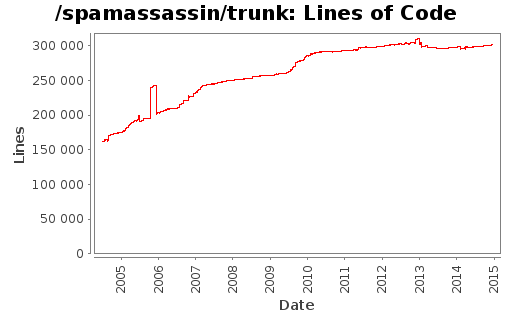
\includegraphics{annexes/lignes.png}[width=1px]
 \caption{Evolution du nombre de ligne de codes}
\end{figure}


\subsection{Q'est ce que SpamAssassin}

SpamAssassin est un programme écrit en PERL dont le but est de filtrer activement les Emails en se basant sur des mécanismes internes. 
SpamAssassin n'effectue aucune action envers les mails, il ajoute seulement des informations personnalisés
qui peuvent être utilisée par d'autres programmes pour effectuer des actions sur les mails (les rangers des dossiers distincts, les supprimer, les bloquer, \dots)


Il peut être utiliser de plusieurs manière:
\begin{itemize}
 \item En mode client, lancé à chaque fois que l'on fait appel à lui
 \item En mode demon grâce à \emph{smapd} , les appels au demon étant fait avec l'utilitaire \emph{spamc}.
 \item Comme une interface de programation: des programmes qui nécéssitent des fonctionnalitées de filtrage de SPAM peuvent s'interfacer avec SpamAssin
 pour construire des solutions utilisant ses fonctionnalités
\end{itemize}

\pagebreak

\section{Ses fonctionnalités}

\subsection{Comment il filtre}

\begin{description}
 \item [Champs d'entête] En se basant sur la forme des entêtes et en les comparant avec des schéma connus par SpamAssasin. En effet 
 on peut se base sur la façon dont certains systèmes de SPAMs construisent leurs messages pour les filtrer. 
 \item [Corps du message] Bien sur SpamAssasin permet de filtrer les mails suivant les mots et expressions qu'ils contiennent. 
 ``ceci n'est pas un SPAM'', ``Bonjour jes suis une princesse d'un royaume africain'', ``Venez chechez votre lot'', \dots sont des expressions
 typiques pour des SPAMs. 
 \item [Filtre bayésien] Filtrer les entêtes et le corps d'un message resultera toujours en de multiples faux positifs. C'est ici que le filtarge 
 bayésien se révèle interessant car il va prendre en considération ce que l'on considère comme SPam et non SPAM soit des ``bon mails'' (``HAM'' en anglais).
 Il va ensuite utiliser les repertoires de SPAMs connu et de ``HAM``  connus, pour y identifier les mots et phrases (Définits comme ''Tokens`` en anglais)
 qui n'apparaissent que dans les SPAMs et que dans les ''HAMs``.
 Un token SPAM trouvé resultant d'une hausse du score (voir \ref{score}) SPAM, un token résultant en une baisse de ce niveau. Ce filtrage permet d'être plus précis et d'éviter les faux positifs, 
 en ne se basant sur un mot ou une phrase mais des enssembles. 
 \item [List noire/blanche automatique] SpamAssassin garde automatiquement une liste blanches des .
 
 Comme précédement si une adresse email envois un SPAM, son score augmente. A l'inverse si elle envoie un ''HAM`` son score baisse. 
 
\end{description} 


Spam Assassin effectue sur chaque mail qui lui est donné à traiter une serie de test, qui vont ensuite donner lieu à un score, qui sera indiqué dans un entête si il est considéré comme SPAM. 
Ce résultat sera ensuite utilisé par d'autres programmes pour déterminer des actions à entreprendre.


\subsection{Le score} \label{score}
C'est la base du fonctionnement du programme.  Après avoir effectué une série de test le programme va déterminer une note. 
\pagebreak

\appendix





\end{document}          
